\documentclass[14pt]{extbook}
\usepackage{multicol, enumerate, enumitem, hyperref, color, soul, setspace, parskip, fancyhdr} %General Packages
\usepackage{amssymb, amsthm, amsmath, latexsym, units, mathtools} %Math Packages
\everymath{\displaystyle} %All math in Display Style
% Packages with additional options
\usepackage[headsep=0.5cm,headheight=12pt, left=1 in,right= 1 in,top= 1 in,bottom= 1 in]{geometry}
\usepackage[usenames,dvipsnames]{xcolor}
\usepackage{dashrule}  % Package to use the command below to create lines between items
\newcommand{\litem}[1]{\item#1\hspace*{-1cm}\rule{\textwidth}{0.4pt}}
\pagestyle{fancy}
\lhead{Progress Quiz 6}
\chead{}
\rhead{Version A}
\lfoot{9689-6866}
\cfoot{}
\rfoot{Spring 2021}
\begin{document}

\begin{enumerate}
\litem{
Choose the equation of the function graphed below.
\begin{center}
    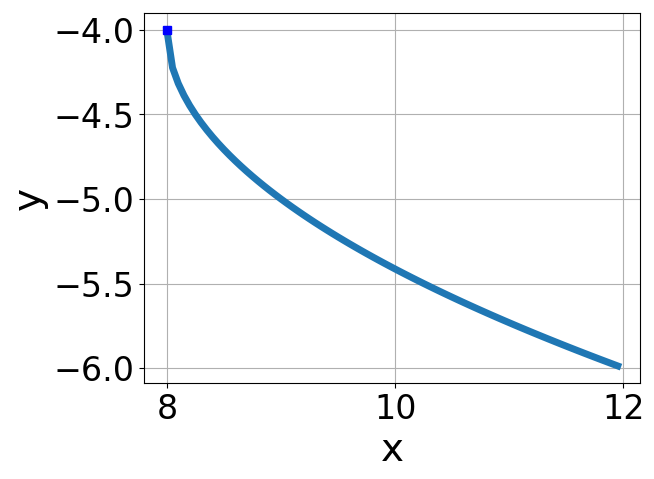
\includegraphics[width=0.5\textwidth]{../Figures/radicalGraphToEquationA.png}
\end{center}
\begin{enumerate}[label=\Alph*.]
\item \( f(x) = - \sqrt[3]{x + 6} + 5 \)
\item \( f(x) = \sqrt[3]{x + 6} + 5 \)
\item \( f(x) = \sqrt[3]{x - 6} + 5 \)
\item \( f(x) = - \sqrt[3]{x - 6} + 5 \)
\item \( \text{None of the above} \)

\end{enumerate} }
\litem{
Choose the graph of the equation below.\[ f(x) = \sqrt{x - 14} - 7 \]\begin{enumerate}[label=\Alph*.]
\begin{multicols}{2}\item 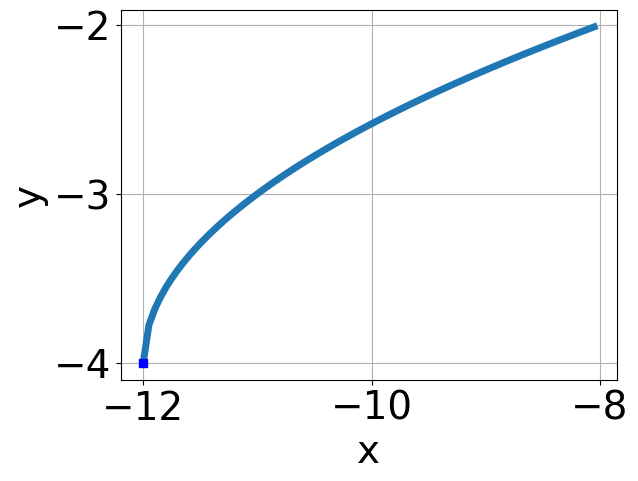
\includegraphics[width = 0.3\textwidth]{../Figures/radicalEquationToGraphCopyAA.png}\item 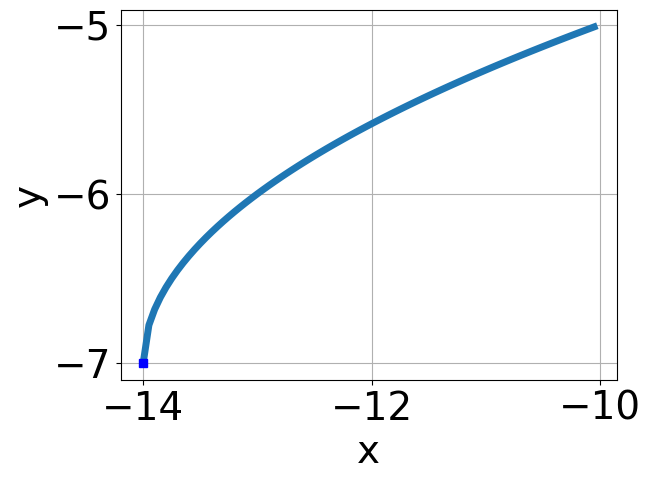
\includegraphics[width = 0.3\textwidth]{../Figures/radicalEquationToGraphCopyBA.png}\item 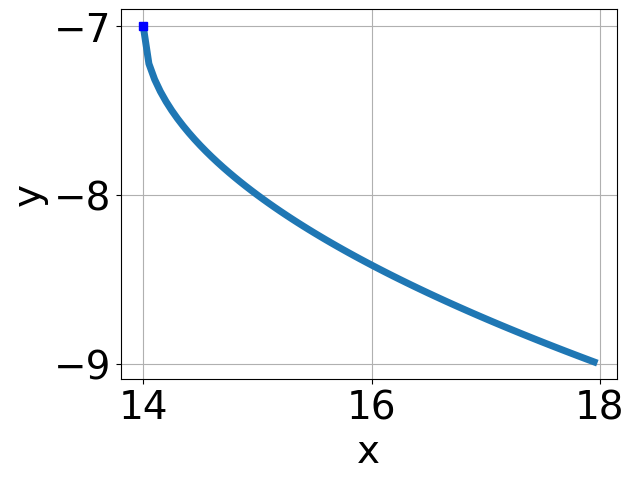
\includegraphics[width = 0.3\textwidth]{../Figures/radicalEquationToGraphCopyCA.png}\item 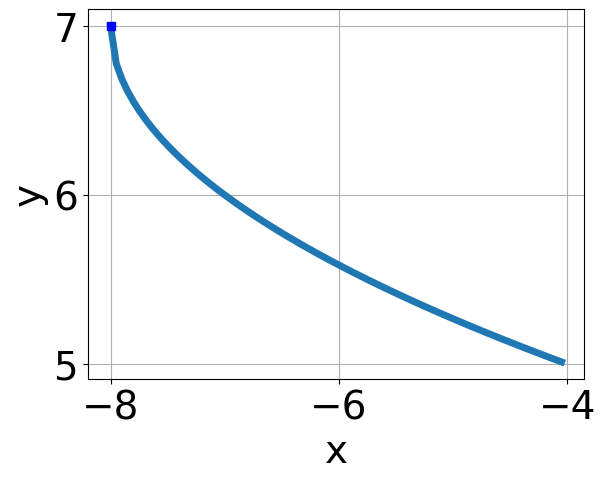
\includegraphics[width = 0.3\textwidth]{../Figures/radicalEquationToGraphCopyDA.png}\end{multicols}\item None of the above.
\end{enumerate} }
\litem{
Choose the graph of the equation below.\[ f(x) = \sqrt[3]{x + 6} - 3 \]\begin{enumerate}[label=\Alph*.]
\begin{multicols}{2}\item 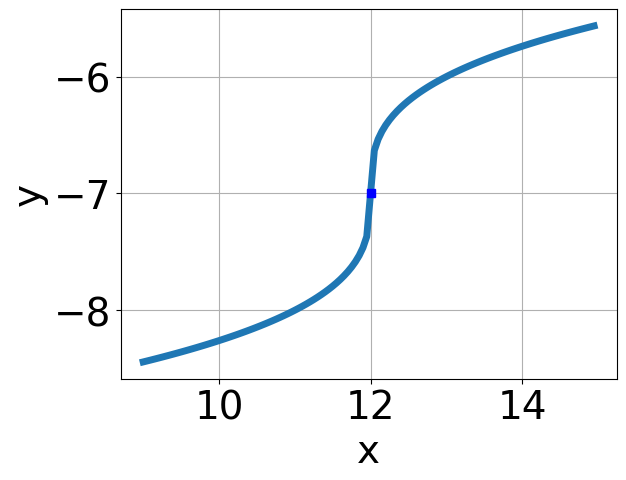
\includegraphics[width = 0.3\textwidth]{../Figures/radicalEquationToGraphAA.png}\item 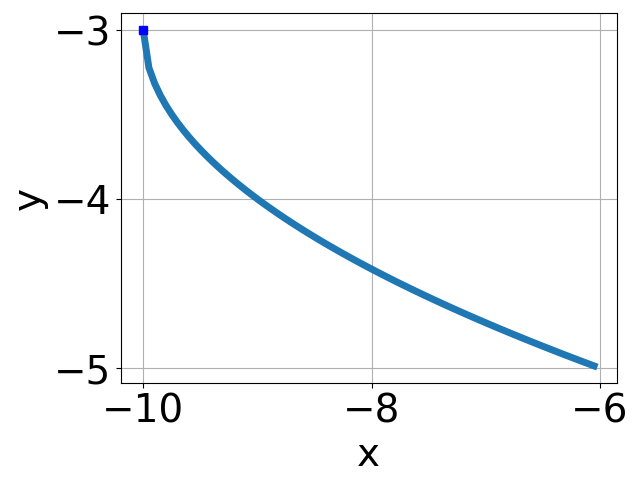
\includegraphics[width = 0.3\textwidth]{../Figures/radicalEquationToGraphBA.png}\item 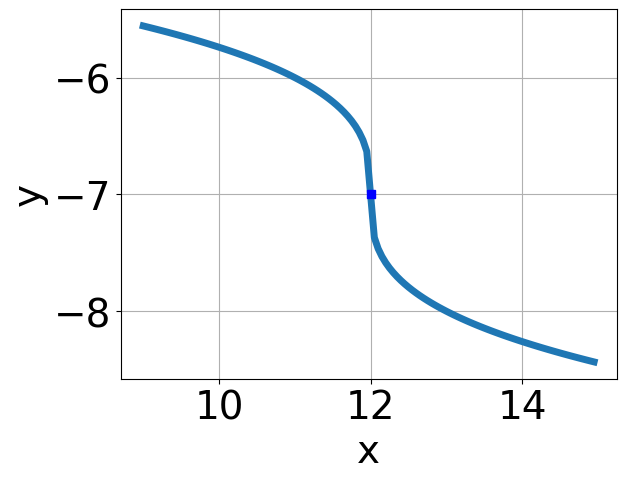
\includegraphics[width = 0.3\textwidth]{../Figures/radicalEquationToGraphCA.png}\item 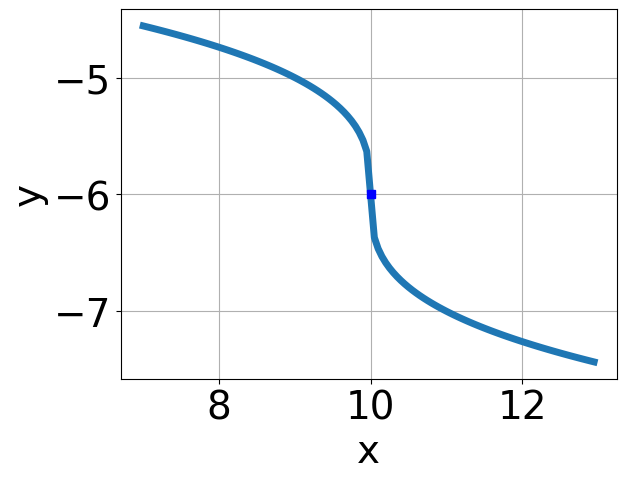
\includegraphics[width = 0.3\textwidth]{../Figures/radicalEquationToGraphDA.png}\end{multicols}\item None of the above.
\end{enumerate} }
\litem{
What is the domain of the function below?\[ f(x) = \sqrt[4]{-8 x - 3} \]\begin{enumerate}[label=\Alph*.]
\item \( (-\infty, a], \text{where } a \in [-3.7, -2.3] \)
\item \( (-\infty, a], \text{ where } a \in [-2, 0.6] \)
\item \( (-\infty, \infty) \)
\item \( [a, \infty), \text{where } a \in [-4.6, -0.5] \)
\item \( [a, \infty), \text{where } a \in [-0.7, -0.2] \)

\end{enumerate} }
\litem{
Choose the equation of the function graphed below.
\begin{center}
    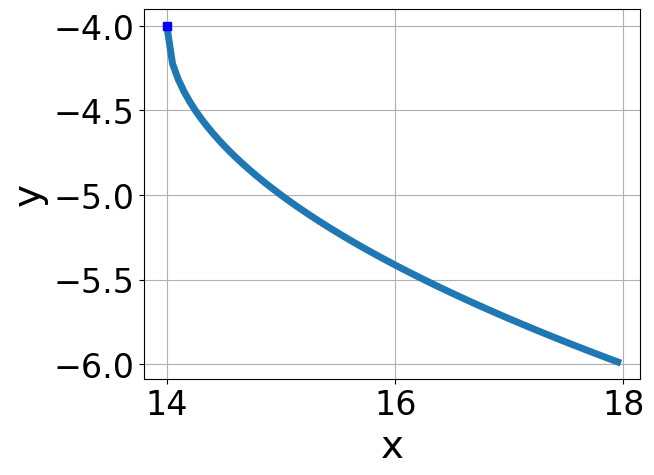
\includegraphics[width=0.5\textwidth]{../Figures/radicalGraphToEquationCopyA.png}
\end{center}
\begin{enumerate}[label=\Alph*.]
\item \( f(x) = - \sqrt{x - 12} - 7 \)
\item \( f(x) = - \sqrt{x + 12} - 7 \)
\item \( f(x) = \sqrt{x + 12} - 7 \)
\item \( f(x) = \sqrt{x - 12} - 7 \)
\item \( \text{None of the above} \)

\end{enumerate} }
\litem{
Solve the radical equation below. Then, choose the interval(s) that the solution(s) belongs to.\[ \sqrt{-54 x^2 - 18} - \sqrt{-93 x} = 0 \]\begin{enumerate}[label=\Alph*.]
\item \( x_1 \in [-0.1, 0.87] \text{ and } x_2 \in [1.2,4.5] \)
\item \( x \in [-0.1,0.87] \)
\item \( x \in [1.3,1.52] \)
\item \( \text{All solutions lead to invalid or complex values in the equation.} \)
\item \( x_1 \in [-0.47, 0.19] \text{ and } x_2 \in [-1.8,-0.6] \)

\end{enumerate} }
\litem{
What is the domain of the function below?\[ f(x) = \sqrt[6]{3 x - 4} \]\begin{enumerate}[label=\Alph*.]
\item \( [a, \infty), \text{where } a \in [0.38, 1.27] \)
\item \( (-\infty, a], \text{where } a \in [0.15, 1.28] \)
\item \( (-\infty, \infty) \)
\item \( [a, \infty), \text{ where } a \in [1.05, 1.39] \)
\item \( (-\infty, a], \text{where } a \in [1.09, 1.6] \)

\end{enumerate} }
\litem{
Solve the radical equation below. Then, choose the interval(s) that the solution(s) belongs to.\[ \sqrt{4 x + 7} - \sqrt{6 x - 6} = 0 \]\begin{enumerate}[label=\Alph*.]
\item \( x_1 \in [-2.8, -0.1] \text{ and } x_2 \in [1,3] \)
\item \( x \in [-0.3,1.2] \)
\item \( \text{All solutions lead to invalid or complex values in the equation.} \)
\item \( x_1 \in [-2.8, -0.1] \text{ and } x_2 \in [4.5,7.5] \)
\item \( x \in [4.3,6.6] \)

\end{enumerate} }
\litem{
Solve the radical equation below. Then, choose the interval(s) that the solution(s) belongs to.\[ \sqrt{9 x - 4} - \sqrt{-8 x - 8} = 0 \]\begin{enumerate}[label=\Alph*.]
\item \( \text{All solutions lead to invalid or complex values in the equation.} \)
\item \( x_1 \in [-2.37, -0.6] \text{ and } x_2 \in [-3.56,4.44] \)
\item \( x \in [-0.6,0.03] \)
\item \( x_1 \in [-0.6, 0.03] \text{ and } x_2 \in [-3.56,4.44] \)
\item \( x \in [0.43,1.39] \)

\end{enumerate} }
\litem{
Solve the radical equation below. Then, choose the interval(s) that the solution(s) belongs to.\[ \sqrt{81 x^2 + 56} - \sqrt{-135 x} = 0 \]\begin{enumerate}[label=\Alph*.]
\item \( x_1 \in [0.67, 0.9] \text{ and } x_2 \in [0.63,1.39] \)
\item \( x \in [-0.94,-0.81] \)
\item \( \text{All solutions lead to invalid or complex values in the equation.} \)
\item \( x \in [-0.8,-0.69] \)
\item \( x_1 \in [-0.94, -0.81] \text{ and } x_2 \in [-0.82,-0.61] \)

\end{enumerate} }
\end{enumerate}

\end{document}